\documentclass{standalone}
\usepackage{preset}
\begin{document}
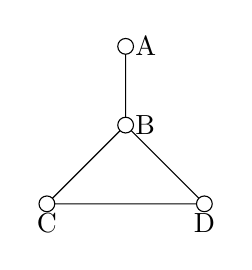
\begin{tikzpicture}[x=20mm,y=20mm]
	\draw(.5,1)--(.5,.5)--(0,0)--(1,0)--(.5,.5);
	\tikzset{every path/.style={draw=black,fill=white}}
	\draw(0,0)circle(.05)node[below]{C};
	\draw(1,0)circle(.05)node[below]{D};
	\draw(.5,.5)circle(.05)node[right]{B};
	\draw(.5,1)circle(.05)node[right]{A};
\end{tikzpicture}
\end{document}
